\documentclass[11pt,a4paper]{article}

\usepackage{amsfonts,amssymb,amsmath}
\usepackage[margin=1in]{geometry}
\usepackage[none]{hyphenat}
\usepackage{graphicx}
\usepackage{fancyhdr}
\usepackage{float}
\usepackage{color}
\usepackage{xcolor}
\usepackage{tikz}
\usepackage[nottoc,notlot,notlof]{tocbibind}

\usetikzlibrary{arrows.meta,shapes,positioning}

\parindent 0ex
% hyphenat[none] forbids hyphenation, so give TeX room to stretch a line
% instead of letting it run into the margin.
\setlength{\emergencystretch}{3em}
\setlength{\parskip}{0.55\baselineskip}
\setlength{\abovedisplayskip}{0.5\baselineskip}
\setlength{\belowdisplayskip}{0.5\baselineskip}
\setlength{\abovedisplayshortskip}{0.25\baselineskip}
\setlength{\belowdisplayshortskip}{0.25\baselineskip}
\numberwithin{equation}{section}

\pagestyle{fancy}
\fancyfoot[C]{\thepage}
\fancyhead{}
\fancyhead[R]{\rightmark}
\renewcommand{\headrulewidth}{0pt}

% Upright operator names; plain italic would read Var as the product V.a.r.
\DeclareMathOperator{\Var}{Var}
\DeclareMathOperator{\Cov}{Cov}
\DeclareMathOperator{\Corr}{Corr}
\DeclareMathOperator{\plim}{plim}
\DeclareMathOperator{\tr}{tr}
\DeclareMathOperator{\rank}{rank}

% Theorem environments.
\usepackage{amsthm}
\theoremstyle{definition}
% One shared counter running section.subsection.n, as in the other courses here.
\newtheorem{thm}{Theorem}[subsection]
\newtheorem{defn}[thm]{Definition}
\newtheorem{exa}[thm]{Example}
\newtheorem{prop}[thm]{Proposition}
\newtheorem{coro}[thm]{Corollary}
\newtheorem{lem}[thm]{Lemma}
% An "In software" panel: the commands, the output they print, and how to read
% it. The web build gives these their own colour (build.py tags the type from
% the label, and "Software" is tested before every other label).
\newtheorem{software}[thm]{Software}
\newtheorem*{note}{Note}
\newtheorem*{remark}{Remark}
\newtheorem{problemx}{Problem}[subsection]
\newenvironment{problem}{\begin{problemx}}{\end{problemx}}
\newenvironment{solution}
  {\renewcommand{\qedsymbol}{}\begin{proof}[\textit{Solution}.]}
  {\end{proof}}
\usepackage{enumitem}
% A heading that is legal inside a theorem body, a list or a float, where
% \subsubsection is not. Same weight as \subsubsection* so the two read alike.
\newcommand{\subhead}[1]{%
  \par\medskip\noindent\textbf{#1}\par\nobreak\smallskip}

\begin{document}
% Title page depersonalised for the web, as with every other course here. The
% identity kept below is the least squares estimator and its covariance matrix,
% which most of the course either derives, tests, or repairs.
\begin{titlepage}
\thispagestyle{empty}
\begin{center}
\vspace*{3cm}
{\Huge\bfseries Econometrics}\\[1.2cm]
{\large Lecture Notes}\\[2.5cm]
\line(1,0){300}\\[1.5cm]
$$b=(X'X)^{-1}X'Y,\qquad \Var(b)=\sigma^{2}(X'X)^{-1}$$
\end{center}
\end{titlepage}

\tableofcontents
\thispagestyle{empty}
\clearpage
\setcounter{page}{1}

%======================================================================
\section{The Nature of Econometrics}
\label{sec:intro}

Economic theory makes statements about how variables are related. The demand for a good falls as its price rises; consumption rises with
income, but by less than income does; output depends on labour and capital. Statements of this kind give the \emph{direction} of an effect and
sometimes its form. They almost never give its \emph{size}. By how much does food consumption fall when its price rises by 10\%? Does a 1\% rise
in capital raise output by more or less than a 1\% rise in labour? Are returns to scale constant? These are quantitative questions, and they
can only be answered from data.

\textbf{Econometrics} is the discipline that answers them. Ragnar Frisch, who coined the word and founded the journal \emph{Econometrica} in 1933,
described it as the unification of three things: economic theory, which says what to look for; mathematics, which states the theory precisely;
and statistics, which confronts the precise statement with data. None of the three is econometrics on its own. Theory without measurement
cannot say how large an effect is. Statistics without theory produces correlations that nobody knows how to interpret.

The defining difficulty of the subject is that economic data are almost never produced by an experiment. A chemist who wants to know the effect
of temperature on a reaction can hold everything else fixed and vary the temperature. An economist who wants to know the effect of a price on
demand must take the prices and quantities that markets happened to produce, in which price, income, tastes and a hundred other things all moved
at once. Much of this course is about the conditions under which such \emph{observational} data can still answer a causal question, and about
what goes wrong when those conditions fail.

\subsection{Economic models and econometric models}
\label{ssec:models}

\begin{defn}
An \textbf{economic model} is a set of assumed relationships among economic variables, usually expressed as equations, together with
restrictions on the signs or sizes of the quantities involved.
\end{defn}

\begin{exa}
\label{ex:keynes}
Keynes's consumption function states that aggregate consumption $C$ depends on disposable income $Y$,
\[
C = f(Y), \qquad 0 < f'(Y) < 1 .
\]
The derivative $f'(Y)$ is the \emph{marginal propensity to consume}: of each additional kwacha of income, some but not all is consumed. In
the simplest version $f$ is linear, $C = \alpha + \beta Y$ with $0 < \beta < 1$.
\end{exa}

The economic model is \emph{exact}: given $Y$, it determines $C$. No data set ever behaves like that. Two households with identical incomes
consume different amounts; the same economy with the same income consumes different amounts in different years. The model must be adapted
before it can be confronted with data, and the adaptation is what turns an economic model into an econometric one.

\begin{defn}
An \textbf{econometric model} consists of
\begin{enumerate}[label=(\roman*)]
\item an equation, or a system of equations, linking observable variables and unobservable \textbf{disturbances}, such as
\[
C_i = \alpha + \beta Y_i + u_i , \qquad i = 1, \dots, n ;
\]
\item a set of assumptions about the joint probability distribution of the disturbances and the explanatory variables, such as
$E(u_i \mid Y_i) = 0$;
\item the set of parameter values regarded as admissible, such as $0 < \beta < 1$.
\end{enumerate}
The process that actually generated the data is the \textbf{data-generating process} (DGP). The model is a family of candidate DGPs indexed by
the parameters, and the task of estimation is to pick out the member of the family that best matches the data.
\end{defn}

The disturbance $u_i$ is not a nuisance added to make the algebra work. It stands for everything that affects $C_i$ besides $Y_i$, and it is
worth listing what that includes, because each item reappears later as a reason the standard assumptions can fail:
\begin{enumerate}[label=(\alph*)]
\item \textbf{Omitted variables.} Wealth, family size, interest rates and expectations all affect consumption. Each is small or hard to
measure, so it is left out and absorbed into $u_i$. If an omitted variable is correlated with $Y_i$, then $E(u_i \mid Y_i) \neq 0$ and the
least squares estimator is biased; the proof comes with the treatment of specification error.
\item \textbf{Measurement error.} National accounts and household surveys measure $C$ and $Y$ imperfectly. Error in the dependent variable
goes into $u_i$ harmlessly; error in the explanatory variable does not, and is one of the main reasons for instrumental variables.
\item \textbf{Functional form.} The true relation may not be linear. The difference between the truth and its linear approximation is part
of $u_i$, and it depends on $Y_i$.
\item \textbf{Intrinsic randomness.} Human behaviour is not fully predictable even when everything measurable is held fixed.
\end{enumerate}

\begin{exa}
\label{ex:cobb}
The Cobb--Douglas production function relates output $Q$ to labour $L$ and capital $K$ by
\[
Q = A L^{\beta_L} K^{\beta_K} e^{u} .
\]
It is not linear in the parameters, but its logarithm is:
\begin{equation}
\label{eq:cobb}
\log Q = \alpha + \beta_L \log L + \beta_K \log K + u , \qquad \alpha = \log A .
\end{equation}
The coefficients are \emph{elasticities}. Holding $K$ fixed,
\[
\beta_L = \frac{\partial \log Q}{\partial \log L} = \frac{\partial Q / Q}{\partial L / L},
\]
the percentage change in output per 1\% change in labour. Scaling both inputs by $\lambda$ multiplies output by
$\lambda^{\beta_L + \beta_K}$, so returns to scale are increasing, constant or decreasing as $\beta_L + \beta_K$ is greater than, equal to or less
than $1$. ``Are returns to scale constant?'' becomes the testable restriction $\beta_L + \beta_K = 1$, a linear restriction of the kind
treated with inference in the $k$-variable model.

Notice that the disturbance entered the original equation \emph{multiplicatively}, as $e^{u}$. That is a modelling choice, made so that the
logarithm produces an additive error. Had the model been $Q = A L^{\beta_L} K^{\beta_K} + u$, taking logarithms would not have produced
\eqref{eq:cobb}, and the model would have had to be estimated by non-linear methods. How the disturbance enters is part of the specification,
not an afterthought.
\end{exa}

\subhead{What econometricians do with a model}
Any empirical study cycles through the same four tasks (Figure~\ref{fig:cycle}).
\begin{enumerate}[label=(\arabic*)]
\item \textbf{Specification}: choose the variables, the functional form and the assumptions on the disturbances.
\item \textbf{Estimation}: use the data to estimate the parameters, by least squares, maximum likelihood, instrumental variables or the
generalised method of moments.
\item \textbf{Evaluation}: test the hypotheses of interest, and test the model itself. Are the residuals consistent with the assumptions? Is
the model stable over time? If not, return to step (1).
\item \textbf{Use}: forecast, or evaluate a policy. What happens to food consumption if a subsidy lowers the price by 10\%?
\end{enumerate}

\begin{figure}[H]
\centering
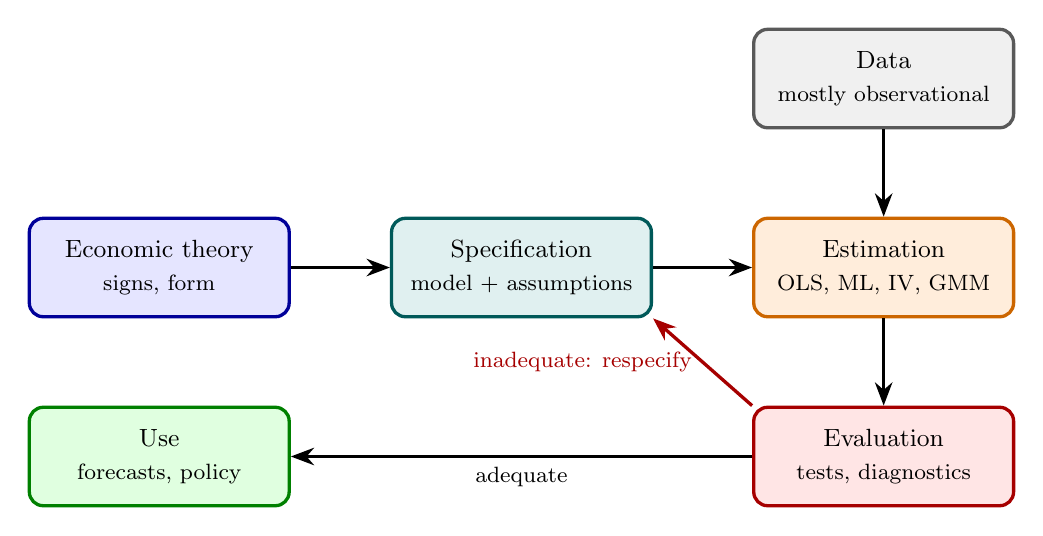
\begin{tikzpicture}[
  box/.style={draw,very thick,rounded corners=5pt,minimum width=3.3cm,minimum height=1.25cm,align=center,font=\small},
  arr/.style={-Stealth,very thick}]
\node[box,fill=blue!10,draw=blue!60!black] (T) at (0,2.4) {Economic theory\\[1pt]\footnotesize signs, form};
\node[box,fill=teal!12,draw=teal!70!black] (S) at (4.6,2.4) {Specification\\[1pt]\footnotesize model + assumptions};
\node[box,fill=orange!14,draw=orange!80!black] (E) at (9.2,2.4) {Estimation\\[1pt]\footnotesize OLS, ML, IV, GMM};
\node[box,fill=gray!12,draw=gray!70!black] (D) at (9.2,4.8) {Data\\[1pt]\footnotesize mostly observational};
\node[box,fill=red!10,draw=red!65!black] (V) at (9.2,0) {Evaluation\\[1pt]\footnotesize tests, diagnostics};
\node[box,fill=green!12,draw=green!50!black] (U) at (0,0) {Use\\[1pt]\footnotesize forecasts, policy};
\draw[arr] (T) -- (S);
\draw[arr] (S) -- (E);
\draw[arr] (D) -- (E);
\draw[arr] (E) -- (V);
\draw[arr] (V) -- node[below,font=\footnotesize] {adequate} (U);
\draw[arr,red!65!black] (V.north west) -- node[left,font=\footnotesize,pos=0.5] {inadequate: respecify} (S.south east);
\end{tikzpicture}
\caption{The cycle of an empirical study. Evaluation either sends the model back to be respecified or releases it for use. The data enter
at the estimation stage.}
\label{fig:cycle}
\end{figure}

\subhead{Causal and predictive questions}
Two different questions can be asked of the same data, and it matters which one is being asked.

A \emph{predictive} question asks what value of $C$ to expect for a household with income $Y$. Any feature of the joint distribution of $C$ and
$Y$ that helps prediction is legitimate, whatever its cause.

A \emph{causal} question asks what would happen to a household's consumption if its income were raised by one kwacha, \emph{other things
equal}. The phrase \emph{ceteris paribus} is the heart of it. In observational data, households with higher incomes also differ in education,
age, location and wealth, and a comparison across households mixes the effect of income with the effects of everything that comes with it.

\begin{exa}
\label{ex:wages}
Regress the log wage of workers on their years of schooling. The slope estimates by how much log wages differ between workers whose schooling
differs by a year. It does not, without more assumptions, estimate the effect of an extra year of schooling on a given worker's wage. Workers
who stay longer at school may differ in ability or family background, and these raise wages directly. Ability is unobserved, so it sits in the
disturbance, and it is correlated with schooling. The comparison across workers then credits schooling with part of the effect of ability. The
slope answers the predictive question correctly and the causal question with a bias. The sections on instrumental variables and on panel data return to this
example with methods that can remove the bias.
\end{exa}

\subsection{Types of economic data}
\label{ssec:data}

The structure of a data set determines which assumptions are plausible and which methods apply, so it is the first thing to settle about
any data set.

\begin{defn}
\label{def:data}
\begin{enumerate}[label=(\roman*)]
\item \textbf{Cross-sectional data} are observations on many units (households, firms, districts, countries) at a single point or period of
time. The units are written $i = 1, \dots, n$ and the order in which they are listed carries no information.
\item \textbf{Time series data} are observations on one unit at successive points in time, $t = 1, \dots, T$, usually equally spaced (annual,
quarterly, monthly, daily). The order is essential.
\item \textbf{Pooled cross sections} combine two or more cross sections drawn independently at different times. Each period has its own sample
of units, and the same unit is not, in general, observed twice.
\item \textbf{Panel (longitudinal) data} follow the \emph{same} units over several periods, giving observations $y_{it}$ with
$i = 1, \dots, n$ and $t = 1, \dots, T$.
\end{enumerate}
\end{defn}

\begin{exa}
\begin{enumerate}[label=(\roman*)]
\item The Living Conditions Monitoring Survey of a given year records the income, expenditure and household size of several thousand Zambian
households: a \emph{cross section}.
\item Annual copper production in Zambia from 1964 to the present, or the monthly consumer price index: \emph{time series}.
\item Two rounds of the household survey, each drawing a fresh random sample of households, combined into one data set to see whether the
relation between income and food expenditure changed between the rounds: \emph{pooled cross sections}.
\item The investment, market value and capital stock of the same ten firms recorded every year for twenty years: a \emph{panel}. So is a
survey that revisits the same households in successive years.
\end{enumerate}
\end{exa}

\begin{figure}[H]
\centering
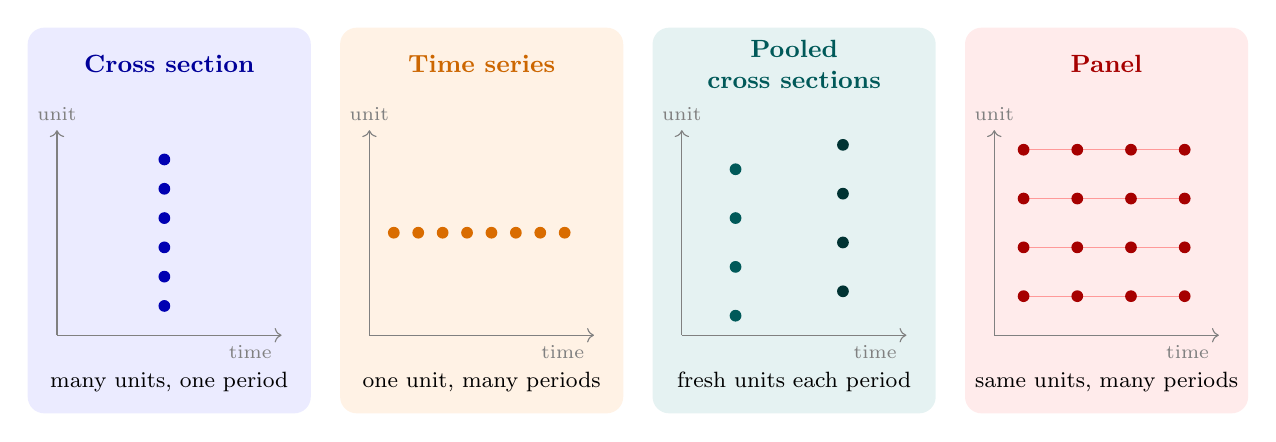
\begin{tikzpicture}[scale=0.62,
  dot/.style={circle,fill,inner sep=1.5pt},
  ttl/.style={font=\small\bfseries,align=center},
  capt/.style={font=\footnotesize,align=center}]
% panel 1: cross section
\begin{scope}[shift={(0,0)}]
\fill[blue!8,rounded corners=6pt] (-0.6,-1.6) rectangle (5.2,6.3);
\node[ttl,blue!60!black] at (2.3,5.55) {Cross section};
\draw[->,gray] (0,0) -- (4.6,0) node[below left,font=\scriptsize] {time};
\draw[->,gray] (0,0) -- (0,4.2) node[above,font=\scriptsize] {unit};
\foreach \y in {0.6,1.2,...,3.6} \node[dot,blue!70!black] at (2.2,\y) {};
\node[capt] at (2.3,-0.95) {many units, one period};
\end{scope}
% panel 2: time series
\begin{scope}[shift={(6.4,0)}]
\fill[orange!10,rounded corners=6pt] (-0.6,-1.6) rectangle (5.2,6.3);
\node[ttl,orange!80!black] at (2.3,5.55) {Time series};
\draw[->,gray] (0,0) -- (4.6,0) node[below left,font=\scriptsize] {time};
\draw[->,gray] (0,0) -- (0,4.2) node[above,font=\scriptsize] {unit};
\foreach \x in {0.5,1.0,...,4.0} \node[dot,orange!85!black] at (\x,2.1) {};
\node[capt] at (2.3,-0.95) {one unit, many periods};
\end{scope}
% panel 3: pooled cross sections
\begin{scope}[shift={(12.8,0)}]
\fill[teal!10,rounded corners=6pt] (-0.6,-1.6) rectangle (5.2,6.3);
\node[ttl,teal!70!black] at (2.3,5.55) {Pooled\\cross sections};
\draw[->,gray] (0,0) -- (4.6,0) node[below left,font=\scriptsize] {time};
\draw[->,gray] (0,0) -- (0,4.2) node[above,font=\scriptsize] {unit};
\foreach \y in {0.4,1.4,2.4,3.4} \node[dot,teal!70!black] at (1.1,\y) {};
\foreach \y in {0.9,1.9,2.9,3.9} \node[dot,teal!40!black] at (3.3,\y) {};
\node[capt] at (2.3,-0.95) {fresh units each period};
\end{scope}
% panel 4: panel
\begin{scope}[shift={(19.2,0)}]
\fill[red!8,rounded corners=6pt] (-0.6,-1.6) rectangle (5.2,6.3);
\node[ttl,red!65!black] at (2.3,5.55) {Panel};
\draw[->,gray] (0,0) -- (4.6,0) node[below left,font=\scriptsize] {time};
\draw[->,gray] (0,0) -- (0,4.2) node[above,font=\scriptsize] {unit};
\foreach \y in {0.8,1.8,2.8,3.8} {
  \draw[red!40] (0.6,\y) -- (3.9,\y);
  \foreach \x in {0.6,1.7,2.8,3.9} \node[dot,red!65!black] at (\x,\y) {};
}
\node[capt] at (2.3,-0.95) {same units, many periods};
\end{scope}
\end{tikzpicture}
\caption{The four data structures, each drawn as observations on a grid of units (vertical) against time (horizontal). Only the panel joins
the same unit across periods.}
\label{fig:datatypes}
\end{figure}

\subhead{Why the distinction matters}
\begin{itemize}
\item In a random cross section the observations are independent, because the units were drawn independently. Their disturbances may have
different variances, since a large household's spending varies more than a small one's. Heteroscedasticity is typically a
cross-section problem.
\item Successive observations in a time series are almost never independent: this year's consumption is close to last year's. Dependence
over time (autocorrelation), trends and unit roots are time-series problems, and asymptotic theory for dependent data replaces the
textbook theory for independent samples.
\item A panel observes each unit repeatedly, so it can separate a unit's permanent characteristics from the effect of the variables that
change over time. Unobserved ability in Example~\ref{ex:wages} is fixed for a worker; with panel data it can be differenced away
with panel methods. Neither a cross section nor a pooled cross section can do this.
\end{itemize}

Two further distinctions recur. \emph{Experimental} data come from a design in which the investigator assigns the explanatory variable at
random; \emph{observational} data do not. And variables are either \emph{flows}, measured over a period (income, consumption, output), or
\emph{stocks}, measured at a point (capital, wealth, money supply). Mixing a stock with a flow requires care about timing: the capital stock
that produced this year's output is the one at the start of the year.

\subhead{Notation}
Throughout, $Y$ is the dependent variable and $X$ an explanatory variable (regressor). A subscript $i$ indexes cross-section units and $t$
indexes time. Lower-case letters denote deviations from sample means,
\[
x_i = X_i - \bar X, \qquad y_i = Y_i - \bar Y ,
\]
a convention that makes the formulas of the two-variable model much shorter. From the treatment of the $k$-variable model onwards the observations are stacked into the
vector $Y$ and the matrix $X$, and the model is written $Y = X\beta + U$. In matrix sections $Y$, $X$ and $U$ denote these arrays; the meaning
is always clear from the context.

\subsection{Describing a bivariate relationship}
\label{ssec:corr}

Before any model is fitted, the relation between two variables is described by its scatter plot and by summary statistics. Given $n$ pairs
$(X_i, Y_i)$, the sample variances and covariance are
\[
s_X^2 = \frac{1}{n-1}\sum x_i^2, \qquad s_Y^2 = \frac{1}{n-1}\sum y_i^2, \qquad s_{XY} = \frac{1}{n-1}\sum x_i y_i .
\]
The covariance has the units of $X$ times $Y$, so its size means nothing on its own. Dividing by the standard deviations removes the units.

\begin{defn}
The \textbf{sample correlation coefficient} of $X$ and $Y$ is
\[
r = \frac{s_{XY}}{s_X s_Y} = \frac{\sum x_i y_i}{\sqrt{\sum x_i^2}\sqrt{\sum y_i^2}} .
\]
\end{defn}

\begin{thm}
\label{thm:cs}
For any real numbers $x_1, \dots, x_n$ and $y_1, \dots, y_n$,
\begin{equation}
\label{eq:cs}
\Bigl(\sum x_i y_i\Bigr)^2 \leq \sum x_i^2 \sum y_i^2 ,
\end{equation}
with equality if and only if one sequence is a multiple of the other. Consequently $-1 \leq r \leq 1$, and $|r| = 1$ if and only if the points
$(X_i, Y_i)$ lie exactly on a straight line.
\end{thm}

\begin{proof}
If every $x_i = 0$ both sides of \eqref{eq:cs} are zero. Otherwise $\sum x_i^2 > 0$ and, for every real $\lambda$,
\[
0 \leq \sum (y_i - \lambda x_i)^2 = \sum y_i^2 - 2\lambda \sum x_i y_i + \lambda^2 \sum x_i^2 .
\]
A quadratic in $\lambda$ with positive leading coefficient that is never negative has at most one real root, so its discriminant is not positive:
\[
4\Bigl(\sum x_i y_i\Bigr)^2 - 4 \sum x_i^2 \sum y_i^2 \leq 0 ,
\]
which is \eqref{eq:cs}. Equality holds exactly when the quadratic has a real root $\lambda_0$, that is when $\sum (y_i - \lambda_0 x_i)^2 = 0$,
which forces $y_i = \lambda_0 x_i$ for every $i$.

Dividing \eqref{eq:cs} by $\sum x_i^2 \sum y_i^2$ gives $r^2 \leq 1$. Equality means $Y_i - \bar Y = \lambda_0 (X_i - \bar X)$ for all $i$, a straight line
through $(\bar X, \bar Y)$ with slope $\lambda_0$, and then $r$ has the sign of $\lambda_0$.
\end{proof}

\begin{coro}
\label{coro:cs}
The quantity $\sum x_i^2 \sum y_i^2 - \bigl(\sum x_i y_i\bigr)^2$ can never be negative. It is zero only when the data lie exactly on a line.
\end{coro}

This corollary settles a question that appears regularly in examinations: a claim that
$\sum (X - \bar X)^2 \sum (Y - \bar Y)^2 - \bigl(\sum (X - \bar X)(Y - \bar Y)\bigr)^2 = -75$ cannot be true for any data set, whatever the
numbers.

\begin{thm}
\label{thm:corrinv}
Let $X_i^* = a + bX_i$ and $Y_i^* = c + dY_i$ with $b \neq 0$ and $d \neq 0$. Then $r_{X^*Y^*} = \operatorname{sgn}(bd)\, r_{XY}$.
\end{thm}

\begin{proof}
The deviations are $x_i^* = b x_i$ and $y_i^* = d y_i$, since the constants $a$ and $c$ cancel against their means. Hence
\[
r_{X^*Y^*} = \frac{bd \sum x_i y_i}{|b|\sqrt{\sum x_i^2}\;|d|\sqrt{\sum y_i^2}} = \frac{bd}{|bd|}\, r_{XY} . \qedhere
\]
\end{proof}

So the correlation between consumption and income is the same whether they are measured in kwacha or in thousands of dollars, and whether or
not an inflation adjustment adds a constant. It changes sign only if one variable is reversed.

\subhead{What a correlation does not measure}
The correlation measures \emph{linear} association and nothing else. If $X$ takes the values $-2, -1, 0, 1, 2$ and $Y = X^2$, then $Y$ is an exact
function of $X$, yet $\sum x_i y_i = \sum X_i^3 - n\bar X \bar Y = 0$ and $r = 0$. A correlation near zero does not mean the variables are
unrelated, and one near $\pm 1$ does not mean a straight line is the right model: a curved relation can also produce a high $r$. Neither
does a correlation say anything about cause. Two series that both grow over time are highly correlated whether or not either affects the other
(Problem~\ref{prob:longley}); this is the problem of spurious regression, studied with unit roots.

\begin{exa}
\label{ex:lcs}
The data set \texttt{LifeCycleSavings}, assembled by Belsley, Kuh and Welsch from earlier work by Sterling, records for 50 countries the
average over 1960--1970 of the aggregate personal savings rate \texttt{sr} (savings as a percentage of disposable income) and of the share of
the population under 15, \texttt{pop15}. The life-cycle hypothesis of Modigliani predicts that a country with more dependants saves less:
children consume without earning. Figure~\ref{fig:lcs} supports the prediction, and the sample correlation is $r = -0.456$.
\end{exa}

\begin{figure}[H]
\centering
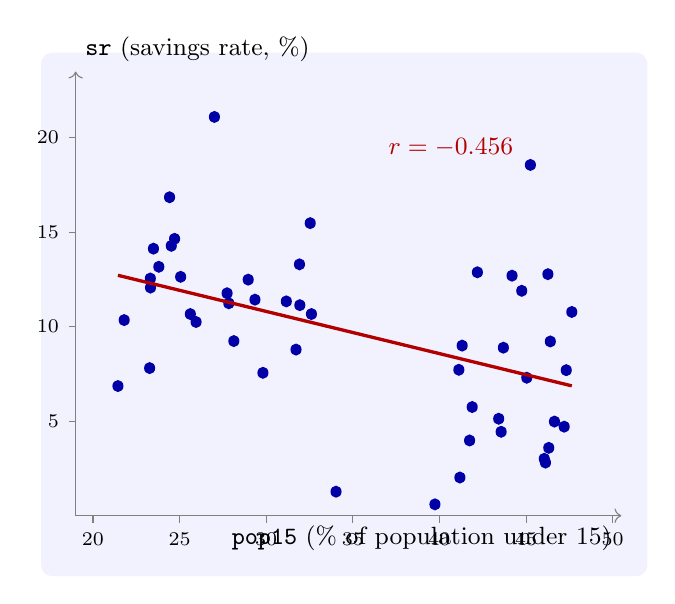
\begin{tikzpicture}[x=0.22cm,y=0.24cm]
\fill[blue!5,rounded corners=4pt] (17,-3.2) rectangle (52,24.5);
\draw[->,gray] (19,0) -- (50.5,0) node[below left,font=\small,black] {\texttt{pop15} (\% of population under 15)};
\draw[->,gray] (19,0) -- (19,23.5) node[above right,font=\small,black] {\texttt{sr} (savings rate, \%)};
\foreach \x in {20,25,...,50} \draw[gray] (\x,0) -- (\x,-0.4) node[below,font=\scriptsize,black] {\x};
\foreach \y in {5,10,15,20} \draw[gray] (19,\y) -- (18.6,\y) node[left,font=\scriptsize,black] {\y};
\foreach \p in {(29.35,11.43), (23.32,12.07), (23.8,13.17), (41.89,5.75), (42.19,12.88), (31.72,8.79), (39.74,0.6), (44.75,11.9),
 (46.64,4.98), (47.64,10.78), (24.42,16.85), (46.31,3.59), (27.84,11.24), (25.06,12.64), (23.31,12.55), (25.62,10.67), (46.05,3.01),
 (47.32,7.7), (34.03,1.27), (41.31,9), (31.16,11.34), (24.52,14.28), (27.01,21.1), (41.74,3.98), (21.8,10.35), (32.54,15.48),
 (25.95,10.25), (24.71,14.65), (32.61,10.67), (45.04,7.3), (43.56,4.44), (41.18,2.02), (44.19,12.7), (46.26,12.78), (28.96,12.49),
 (31.94,11.14), (31.92,13.3), (27.74,11.77), (21.44,6.86), (23.49,14.13), (43.42,5.13), (46.12,2.81), (23.27,7.81), (29.81,7.56),
 (46.4,9.22), (45.25,18.56), (41.12,7.72), (28.13,9.24), (43.69,8.89), (47.2,4.71)}
  \fill[blue!65!black] \p circle (0.32);
\draw[very thick,red!70!black] (21.44,12.72) -- (47.64,6.87);
\node[red!70!black,font=\small,align=left,anchor=west] at (36.5,19.5) {$r = -0.456$};
\end{tikzpicture}
\caption{Savings rate against the share of the population under 15, for 50 countries, 1960--1970 averages. The line is the least squares fit
of the two-variable model, drawn here only as a guide to the eye.}
\label{fig:lcs}
\end{figure}

\subsection{The conditional expectation function}
\label{ssec:cef}

A scatter plot is a sample. Behind it stands a population joint distribution of $(X, Y)$, and the object that regression analysis estimates
is a feature of that distribution. It is worth being precise about which feature, because the answer explains both what regression can do
without any assumptions and what it needs assumptions for.

\begin{defn}
Let $(X, Y)$ be random variables with $E(Y^2) < \infty$. The \textbf{conditional expectation function} (CEF) of $Y$ given $X$ is
$m(x) = E(Y \mid X = x)$. The random variable $m(X) = E(Y \mid X)$ is the CEF evaluated at $X$.
\end{defn}

The proofs below use two properties of conditional expectation, which hold whenever the expectations exist: the \emph{law of iterated
expectations} $E\bigl[E(Y \mid X)\bigr] = E(Y)$, and the fact that a function of $X$ can be taken outside a conditional expectation given $X$,
$E\bigl[h(X) Y \mid X\bigr] = h(X)\, E(Y \mid X)$.

\begin{thm}[CEF decomposition]
\label{thm:cefdecomp}
Every $Y$ with finite variance can be written
\[
Y = m(X) + \varepsilon , \qquad \varepsilon = Y - E(Y \mid X),
\]
where
\begin{enumerate}[label=(\roman*)]
\item $E(\varepsilon \mid X) = 0$, and hence $E(\varepsilon) = 0$;
\item $\varepsilon$ is uncorrelated with every function $h(X)$ for which $E\bigl[h(X)^2\bigr] < \infty$.
\end{enumerate}
\end{thm}

\begin{proof}
(i) $E(\varepsilon \mid X) = E(Y \mid X) - E\bigl[m(X) \mid X\bigr] = m(X) - m(X) = 0$. Taking expectations,
$E(\varepsilon) = E\bigl[E(\varepsilon \mid X)\bigr] = 0$.

(ii) By iterated expectations and (i),
\[
E\bigl[h(X)\varepsilon\bigr] = E\Bigl[E\bigl(h(X)\varepsilon \mid X\bigr)\Bigr] = E\bigl[h(X)\, E(\varepsilon \mid X)\bigr] = 0 .
\]
Since $E(\varepsilon) = 0$, $\Cov\bigl(h(X), \varepsilon\bigr) = E\bigl[h(X)\varepsilon\bigr] = 0$.
\end{proof}

The theorem says something striking: the decomposition into ``systematic part'' and ``disturbance with conditional mean zero'' is not an
assumption about the world. It is always available, by construction. What \emph{is} an assumption is that $m(x)$ has a particular form, say
$\alpha + \beta x$, and, for causal work, that $m$ describes what happens when $X$ is changed rather than merely what is observed alongside it.

\begin{thm}[The CEF is the best predictor]
\label{thm:cefbest}
Among all functions $g$ with $E\bigl[g(X)^2\bigr] < \infty$, the mean squared prediction error $E\bigl[\bigl(Y - g(X)\bigr)^2\bigr]$ is minimised by
$g = m$.
\end{thm}

\begin{proof}
Write $Y - g(X) = \bigl(Y - m(X)\bigr) + \bigl(m(X) - g(X)\bigr) = \varepsilon + h(X)$, where $h = m - g$ is a function of $X$. Then
\begin{align*}
E\bigl[\bigl(Y - g(X)\bigr)^2\bigr] &= E(\varepsilon^2) + 2E\bigl[h(X)\varepsilon\bigr] + E\bigl[h(X)^2\bigr]\\
&= E(\varepsilon^2) + E\bigl[h(X)^2\bigr],
\end{align*}
because the cross term is zero by Theorem~\ref{thm:cefdecomp}(ii). The first term does not depend on $g$ and the second is non-negative and
zero when $g = m$.
\end{proof}

The CEF may be any function at all. If attention is restricted to \emph{linear} predictors, the best one has an explicit formula.

\begin{thm}[Best linear predictor]
\label{thm:blp}
Let $\Var(X) > 0$. The values of $a$ and $b$ minimising $E\bigl[(Y - a - bX)^2\bigr]$ are
\[
b^* = \frac{\Cov(X, Y)}{\Var(X)}, \qquad a^* = E(Y) - b^* E(X) .
\]
The error $v = Y - a^* - b^* X$ satisfies $E(v) = 0$ and $\Cov(X, v) = 0$.
\end{thm}

\begin{proof}
Let $\mu_X = E(X)$ and $\mu_Y = E(Y)$. The objective $S(a, b) = E\bigl[(Y - a - bX)^2\bigr]$ is a convex quadratic in $(a, b)$, so its minimum is
where both partial derivatives vanish:
\[
\frac{\partial S}{\partial a} = -2E(Y - a - bX) = 0, \qquad \frac{\partial S}{\partial b} = -2E\bigl[X(Y - a - bX)\bigr] = 0 .
\]
The first gives $a = \mu_Y - b\mu_X$, which is the statement $E(v) = 0$. Substituting into the second,
\[
E\bigl[X\bigl((Y - \mu_Y) - b(X - \mu_X)\bigr)\bigr] = \Cov(X, Y) - b\Var(X) = 0 ,
\]
since $E\bigl[X(Y - \mu_Y)\bigr] = \Cov(X, Y)$ and $E\bigl[X(X - \mu_X)\bigr] = \Var(X)$. Hence $b = b^*$, and the second equation, with $E(v) = 0$, is
$\Cov(X, v) = 0$. Convexity follows from the Hessian
$2\begin{pmatrix} 1 & \mu_X \\ \mu_X & E(X^2)\end{pmatrix}$, whose determinant $4\Var(X)$ is positive.
\end{proof}

\begin{coro}
\label{coro:linearcef}
If the CEF is linear, $m(x) = \alpha + \beta x$, then $\alpha = a^*$ and $\beta = b^*$: the best linear predictor and the CEF coincide.
\end{coro}

\begin{proof}
If $m$ is linear then $Y = \alpha + \beta X + \varepsilon$ with $E(\varepsilon) = 0$ and $\Cov(X, \varepsilon) = 0$, by Theorem~\ref{thm:cefdecomp}.
These are exactly the two conditions that characterise $(a^*, b^*)$ in the proof of Theorem~\ref{thm:blp}, and the solution of those conditions
is unique because $\Var(X) > 0$.
\end{proof}

The bivariate normal distribution is the leading case of a linear CEF: if $(X, Y)$ is bivariate normal then
$E(Y \mid X = x) = \mu_Y + \rho \frac{\sigma_Y}{\sigma_X}(x - \mu_X)$, a straight line with slope
$\rho\sigma_Y/\sigma_X = \Cov(X, Y)/\Var(X) = b^*$.

\begin{exa}
\label{ex:blp}
Let $X$ be uniform on $(0, 1)$ and $Y = X^2 + \varepsilon$, with $\varepsilon$ independent of $X$, $E(\varepsilon) = 0$. The CEF is $m(x) = x^2$, a curve.
The moments of the uniform distribution are $E(X^k) = \frac{1}{k+1}$, so
\begin{align*}
\Var(X) &= \tfrac13 - \tfrac14 = \tfrac{1}{12},\\
\Cov(X, Y) &= \Cov(X, X^2) = E(X^3) - E(X)E(X^2) = \tfrac14 - \tfrac12\cdot\tfrac13 = \tfrac{1}{12} .
\end{align*}
Hence $b^* = 1$ and $a^* = E(Y) - b^*E(X) = \frac13 - \frac12 = -\frac16$. The best linear predictor is $-\frac16 + x$. It is the straight line that
fits the parabola $x^2$ best on average over $(0, 1)$. It lies above the parabola in the middle of the interval and below it at both ends,
crossing it where $x^2 = x - \frac16$, at $x = \frac12 \pm \frac{1}{2\sqrt3}$, about $0.211$ and $0.789$.

Least squares applied to a large sample from this population estimates $-\frac16 + x$. That is a correct estimate of the best linear
predictor. It is a wrong estimate of the CEF, and the slope $1$ is not ``the effect of $X$'': the true derivative $2x$ ranges from $0$ to $2$.
\end{exa}

The lesson for the rest of the course is that least squares always estimates something well defined, the best linear predictor. Whether that
something is the CEF depends on the functional form, and whether it is a causal effect depends on the assumptions about the
disturbance.

\subsection{The software workflow}
\label{ssec:software}

Modern econometrics is done with software, and a postgraduate economist is expected to be fluent in at least one package. These notes use
\textbf{R}, which is free, runs on every operating system, and records an analysis as a script that anyone can rerun. Every panel marked
\emph{Software} shows commands, the output they actually print, and how to read that output against the theory. Where a command differs
in \textbf{Stata} or \textbf{EViews}, the two other packages most used in economics, the equivalent is given at the end of the panel.

A reproducible analysis has a fixed shape whatever the package:
\begin{enumerate}[label=(\arabic*)]
\item \textbf{Load} the data from a file or a database, never by retyping.
\item \textbf{Inspect}: dimensions, variable names, summary statistics, plots. Most errors in empirical work are data errors found at
this stage or not at all.
\item \textbf{Transform}: logarithms, differences, deflating by a price index. Do it in the script, so the transformation is recorded.
\item \textbf{Estimate and test.}
\item \textbf{Report}, with the script kept alongside the results.
\end{enumerate}
Menu-driven work in Stata or EViews is convenient while exploring. The final analysis should still be a script (a Stata \texttt{do}-file, an
EViews program), because a result that cannot be reproduced cannot be checked.

\begin{software}[Loading and inspecting a cross section]
\label{sw:lcs}
\texttt{LifeCycleSavings} is supplied with R.
{\small\begin{verbatim}
> data(LifeCycleSavings)
> head(LifeCycleSavings, 4)
             sr pop15 pop75     dpi ddpi
Australia 11.43 29.35  2.87 2329.68 2.87
Austria   12.07 23.32  4.41 1507.99 3.93
Belgium   13.17 23.80  4.43 2108.47 3.82
Bolivia    5.75 41.89  1.67  189.13 0.22
> dim(LifeCycleSavings)
[1] 50  5
> summary(LifeCycleSavings$sr)
   Min. 1st Qu.  Median    Mean 3rd Qu.    Max.
  0.600   6.970  10.510   9.671  12.617  21.100
\end{verbatim}}
\textbf{Reading the output.} The data are a cross section: one row per country, 50 rows, and the row order (alphabetical) carries no meaning.
Besides \texttt{sr} and \texttt{pop15} there are \texttt{pop75}, the percentage aged over 75, \texttt{dpi}, real per capita disposable income in
US dollars, and \texttt{ddpi}, its growth rate in percent. The savings rate ranges from $0.6\%$ to $21.1\%$. Its mean, $9.67$, is a little below
its median, $10.51$, a sign of a longer tail on the low side.

\textbf{Stata:} \texttt{summarize sr} (or \texttt{summarize sr, detail} for quartiles). \textbf{EViews:} open the series and choose
\emph{View $\to$ Descriptive Statistics}, or type \texttt{sr.stats}.
\end{software}

\begin{software}[Correlations and a test of zero correlation]
\label{sw:cor}
The correlation matrix of all five variables, then a test that one correlation is zero:
{\small\begin{verbatim}
> round(cor(LifeCycleSavings), 3)
          sr  pop15  pop75    dpi   ddpi
sr     1.000 -0.456  0.317  0.220  0.305
pop15 -0.456  1.000 -0.908 -0.756 -0.048
pop75  0.317 -0.908  1.000  0.787  0.025
dpi    0.220 -0.756  0.787  1.000 -0.129
ddpi   0.305 -0.048  0.025 -0.129  1.000
> with(LifeCycleSavings, cor.test(sr, pop15))

        Pearson's product-moment correlation

data:  sr and pop15
t = -3.5453, df = 48, p-value = 0.0008866
alternative hypothesis: true correlation is not equal to 0
95 percent confidence interval:
 -0.6513020 -0.2029202
sample estimates:
       cor
-0.4555381
\end{verbatim}}
\textbf{Reading the output.} The matrix is symmetric with ones on the diagonal, as Theorem~\ref{thm:cs} requires. Savings are negatively correlated
with the young-dependant share and positively with the old-age share. That second sign is surprising at first, because the elderly also
dissave. The explanation is the very large correlation, $-0.908$, between \texttt{pop15} and \texttt{pop75}: countries with many children have few
old people. Pairwise correlations cannot separate the two effects, and that is what multiple regression is for.

The test in the second command is of $H_0\colon \rho = 0$. Its statistic is
\[
t = \frac{r\sqrt{n-2}}{\sqrt{1 - r^2}} = \frac{-0.4555\sqrt{48}}{\sqrt{1 - 0.2075}} = -3.545 ,
\]
which has a $t_{n-2}$ distribution when $\rho = 0$ and the observations are independent draws from a bivariate normal distribution. It is the
same statistic as the $t$ test on the slope of a two-variable regression. With $p = 0.0009$ the hypothesis of no correlation is
firmly rejected.

The confidence interval is \emph{not} $r \pm 1.96\,\mathrm{se}$. It uses Fisher's transformation $z = \tanh^{-1} r$, which is approximately
normal with variance $\frac{1}{n-3}$. Here $\tanh^{-1}(-0.4555) = -0.4917$, so the interval for $\tanh^{-1}\rho$ is
$-0.4917 \pm 1.96/\sqrt{47} = (-0.7776, -0.2058)$, and applying $\tanh$ to both ends gives the printed $(-0.651, -0.203)$. The interval is
asymmetric about $r$ because the correlation is bounded by $\pm 1$. Why the transformation works is an application of the delta method, proved
with the large-sample theory later in the course.

\textbf{Stata:} \texttt{correlate sr pop15 pop75 dpi ddpi}, and \texttt{pwcorr sr pop15, sig} for the $p$-value. \textbf{EViews:} select the
series, open them as a group and choose \emph{View $\to$ Covariance Analysis}, ticking \emph{Correlation} and \emph{t-statistic}.
\end{software}

\begin{software}[A time series]
\label{sw:ts}
The number of mobile telephone subscribers in Zambia, in thousands, for 2010--2014:
{\small\begin{verbatim}
> subs <- ts(c(38.1, 80.0, 170.4, 354.5, 744.4), start = 2010)
> round(diff(log(subs)), 3)
Time Series:
Start = 2011
End = 2014
Frequency = 1
[1] 0.742 0.756 0.733 0.742
\end{verbatim}}
\textbf{Reading the output.} \texttt{ts} attaches dates, so R knows the order matters. The first difference of the logarithm,
$\log Y_t - \log Y_{t-1} = \log(Y_t/Y_{t-1})$, is the growth rate in continuous terms. It is remarkably steady, close to $0.74$ every year,
which says the series is growing at a \emph{constant proportional rate}. A plot of $\log Y_t$ against $t$ is then a straight line, and fitting
that line is the constant growth curve, the subject of the section on functional form, where these data
are analysed fully.

\textbf{Stata:} \texttt{tsset year}, then \texttt{generate g = D.ln\_subs}. \textbf{EViews:} \texttt{series g = dlog(subs)}.
\end{software}

\subsection{Practice Problems}

\begin{problem}
Define each of the following, with an example:
\begin{enumerate}[label=(\roman*)]
\item cross-sectional data;
\item panel data;
\item pooled cross-sectional data.
\end{enumerate}
Explain why panel data and pooled cross sections, which both have a time dimension and many units, are not the same thing.
\end{problem}

\begin{solution}
(i) Observations on many units at one point or period of time; for example, the incomes and food expenditures of 5\,000 households in a
national survey of a given year. (ii) Observations on the \emph{same} units at several points in time; for example, the annual output, employment
and capital stock of the same 200 manufacturing firms for ten years. (iii) Independent cross sections from different periods combined into one
data set; for example, two household surveys five years apart, each with a fresh random sample.

The difference is whether a unit is followed. In a panel, firm $i$ in year 1 and firm $i$ in year 2 are the same firm, so the data can compare a
unit with itself and remove its permanent unobserved characteristics. In pooled cross sections the households of the two rounds are different
households. The data can compare the two populations, not the units. A pooled cross section is also independent across periods by
construction, while a panel's repeated observations on one unit are typically correlated.
\end{solution}

\begin{problem}
\label{prob:minus75}
For a sample of observations on $X$ and $Y$ a student reports
\[
\sum (X_i - \bar X)^2 \sum (Y_i - \bar Y)^2 - \Bigl(\sum (X_i - \bar X)(Y_i - \bar Y)\Bigr)^2 = -75 .
\]
Can this be correct? Give a reason.
\end{problem}

\begin{solution}
No. By the Cauchy--Schwarz inequality (Theorem~\ref{thm:cs}), $\bigl(\sum x_i y_i\bigr)^2 \leq \sum x_i^2 \sum y_i^2$ for any numbers, so the expression
is always $\geq 0$. Equivalently, it equals $\sum x_i^2 \sum y_i^2 (1 - r^2)$, which is non-negative because $r^2 \leq 1$. A negative value means an
arithmetic error. It is zero only if the points lie exactly on a line.
\end{solution}

\begin{problem}
Two analysts compute the correlation between the price and quantity of maize. One measures price in kwacha per kilogram and quantity in
tonnes; the other measures price in US dollars per 50\,kg bag, after subtracting a transport cost of K15 per bag, and quantity in kilograms. Show that
they obtain the same correlation. Under what transformation of the data would the sign change?
\end{problem}

\begin{solution}
Each change of units is an increasing linear transformation. The dollar price per bag is $(50P - 15)/e$ for an exchange rate of $e$ kwacha
per dollar, of the form $a + bP$ with $b = 50/e > 0$, and kilograms are $1000$ times tonnes. By Theorem~\ref{thm:corrinv}
the correlation is multiplied by $\operatorname{sgn}(bd) = +1$. The sign changes only if exactly one variable is transformed with a negative
slope, for example if quantity were replaced by unsold stock, $S - Q$ for a fixed supply $S$.
\end{solution}

\begin{problem}
Let $X$ take the values $0$, $1$ and $2$ with probability $\frac13$ each, and let $E(Y \mid X) = X^2$.
\begin{enumerate}[label=(\alph*)]
\item Find the best linear predictor $a^* + b^* X$.
\item Find the mean squared difference $E\bigl[(m(X) - a^* - b^* X)^2\bigr]$ between the CEF and the best linear predictor.
\end{enumerate}
\end{problem}

\begin{solution}
(a) The needed moments are $E(X) = 1$, $E(X^2) = \frac53$ and $E(X^3) = \frac{0 + 1 + 8}{3} = 3$. By iterated expectations
$E(Y) = E(X^2) = \frac53$ and $\Cov(X, Y) = \Cov\bigl(X, E(Y \mid X)\bigr) = \Cov(X, X^2) = 3 - 1\cdot\frac53 = \frac43$. Also $\Var(X) = \frac53 - 1 = \frac23$.
Hence $b^* = \frac{4/3}{2/3} = 2$ and $a^* = \frac53 - 2 = -\frac13$.

(The step $\Cov(X, Y) = \Cov\bigl(X, E(Y \mid X)\bigr)$ holds because $E(XY) = E\bigl[X\,E(Y \mid X)\bigr]$ by iterated expectations. The best linear
predictor depends on $Y$ only through its CEF.)

(b) At $X = 0, 1, 2$ the CEF is $0, 1, 4$ and the predictor is $-\frac13, \frac53, \frac{11}{3}$. The differences are $\frac13$, $-\frac23$ and $\frac13$, so
the mean squared difference is $\frac13\bigl(\frac19 + \frac49 + \frac19\bigr) = \frac29$. By the proof of Theorem~\ref{thm:cefbest}, this is exactly how much larger
the mean squared prediction error of the best linear predictor is than that of the CEF.
\end{solution}

\begin{problem}
Let $X$ be symmetric about zero with $E(X^4) < \infty$ and $\Var(X) > 0$, and let $\varepsilon = X^2 - E(X^2)$.
\begin{enumerate}[label=(\alph*)]
\item Show that $E(\varepsilon) = 0$ and $\Cov(X, \varepsilon) = 0$.
\item Show that $E(\varepsilon \mid X) \neq 0$.
\item What does this show about the relation between ``uncorrelated with $X$'' and ``conditional mean zero given $X$''?
\end{enumerate}
\end{problem}

\begin{solution}
(a) $E(\varepsilon) = E(X^2) - E(X^2) = 0$. By symmetry $E(X) = 0$ and $E(X^3) = 0$, so
$\Cov(X, \varepsilon) = E(X\varepsilon) = E(X^3) - E(X)E(X^2) = 0$.

(b) $E(\varepsilon \mid X) = X^2 - E(X^2)$, which is a non-constant function of $X$ because $X$ is not degenerate. It is not identically zero.

(c) Zero conditional mean implies zero correlation with every function of $X$ (Theorem~\ref{thm:cefdecomp}), and in particular with $X$
itself. The converse fails: $\varepsilon$ here is uncorrelated with $X$ but perfectly predictable from $X^2$. The error of a best linear predictor is
always uncorrelated with $X$, by Theorem~\ref{thm:blp}, but it has conditional mean zero only when the CEF is linear. The distinction matters
later: unbiasedness of least squares needs the stronger condition, while consistency needs only the weaker one.
\end{solution}

\begin{problem}
In the Cobb--Douglas model \eqref{eq:cobb}, estimated from 40 observations, the estimates are $\hat\beta_L = 0.7$ and $\hat\beta_K = 0.2$.
\begin{enumerate}[label=(\alph*)]
\item Interpret each estimate.
\item What do the estimates suggest about returns to scale?
\item What further information would be needed to decide whether the data are consistent with constant returns to scale?
\end{enumerate}
\end{problem}

\begin{solution}
(a) Holding capital fixed, a 1\% increase in labour is associated with a $0.7\%$ increase in output. Holding labour fixed, a 1\% increase in
capital is associated with a $0.2\%$ increase in output.

(b) Scaling both inputs by 1\% raises output by about $\hat\beta_L + \hat\beta_K = 0.9\%$, which points to decreasing returns to scale.

(c) $0.9$ is an estimate, so the question is whether it differs from $1$ by more than sampling error. That requires the standard error of
$\hat\beta_L + \hat\beta_K$, which is
$\sqrt{\Var(\hat\beta_L) + \Var(\hat\beta_K) + 2\Cov(\hat\beta_L, \hat\beta_K)}$. The \emph{covariance} of the two estimates is needed as well as
their standard errors. It is usually negative, because labour and capital tend to move together, and it can change the answer. The test of
$\beta_L + \beta_K = 1$ is developed with inference in the $k$-variable model.
\end{solution}

\begin{problem}
\label{prob:longley}
The data set \texttt{longley}, supplied with R, holds annual US data for 1947--1962. In R,
{\small\begin{verbatim}
> with(longley, round(c(cor(Employed, GNP), cor(Employed, Year)), 4))
[1] 0.9836 0.9713
> with(longley, round(cor(diff(Employed), diff(GNP)), 4))
[1] 0.892
\end{verbatim}}
\begin{enumerate}[label=(\alph*)]
\item Employment is almost as highly correlated with the calendar year as with GNP. What does that suggest about the correlation of $0.984$?
\item Why is the correlation of the year-to-year changes a more informative measure of whether employment and output move together?
\item Write the Stata or EViews commands that would compute the correlation of the changes.
\end{enumerate}
\end{problem}

\begin{solution}
(a) Both series grow steadily over the sixteen years. Any two trending series are highly correlated with each other, and each is highly
correlated with time, whether or not they are related. A large part of $0.984$ reflects the common upward trend rather than any connection
between employment and output.

(b) Differencing removes a linear trend: if $Y_t = \alpha + \delta t + e_t$ then $\Delta Y_t = \delta + \Delta e_t$, and the trend leaves only a constant.
The correlation of the changes asks whether employment rises \emph{more than usual} in years when output rises more than usual. Here it is still
$0.892$, so the co-movement is real and not only a shared trend. That conclusion was not available from the levels. The section on unit roots makes this
precise.

(c) Stata: \texttt{tsset Year}, then \texttt{correlate D.Employed D.GNP}. EViews: \texttt{group g d(employed) d(gnp)}, then \texttt{g.cor}.
\end{solution}

\section*{References}
\addcontentsline{toc}{section}{References}

\subhead{Prescribed text}
\begin{enumerate}
\item Johnston, J., and DiNardo, J. (1997), \emph{Econometric Methods} (4th ed.), New York, McGraw-Hill.
\end{enumerate}

\subhead{Recommended texts}
\begin{enumerate}
\item Davidson, R., and MacKinnon, J. G. (2004), \emph{Econometric Theory and Methods}, New York, Oxford University Press.
\item Greene, W. H. (2018), \emph{Econometric Analysis} (8th ed.), New York, Pearson.
\item Hayashi, F. (2000), \emph{Econometrics}, Princeton, Princeton University Press.
\item Wooldridge, J. M. (2010), \emph{Econometric Analysis of Cross Section and Panel Data} (2nd ed.), Cambridge, MA, MIT Press.
\end{enumerate}

\subhead{Software}
\begin{enumerate}
\item Kleiber, C., and Zeileis, A. (2008), \emph{Applied Econometrics with R}, New York, Springer.
\item R Core Team, \emph{R: A Language and Environment for Statistical Computing}, Vienna, R Foundation for Statistical Computing,
\texttt{https://www.R-project.org}.
\end{enumerate}

\subhead{Further reading}
\begin{enumerate}
\item Angrist, J. D., and Pischke, J.-S. (2009), \emph{Mostly Harmless Econometrics}, Princeton, Princeton University Press.
\item Anscombe, F. J. (1973), Graphs in statistical analysis, \emph{The American Statistician}, 27, 17--21.
\item Belsley, D. A., Kuh, E., and Welsch, R. E. (1980), \emph{Regression Diagnostics}, New York, Wiley.
\item Frisch, R. (1933), Editor's note, \emph{Econometrica}, 1, 1--4.
\item Haavelmo, T. (1944), The probability approach in econometrics, \emph{Econometrica}, 12 (Supplement), 1--118.
\item Modigliani, F. (1966), The life cycle hypothesis of saving, the demand for wealth and the supply of capital, \emph{Social Research}, 33,
160--217.
\end{enumerate}

\end{document}
